% Borrador del artículo — plantilla genérica.
% Cuando se elija la revista (RIAI o MDPI), migrar el contenido de secciones/ a su plantilla oficial.
\documentclass[11pt,a4paper]{article}
\usepackage[utf8]{inputenc}
\usepackage[T1]{fontenc}
\usepackage[english,spanish,es-tabla,es-nodecimaldot]{babel}
\usepackage{lmodern}
\usepackage{microtype}
\usepackage[margin=2.5cm]{geometry}
\usepackage{graphicx}
\usepackage{booktabs}
\usepackage{siunitx}
\usepackage{listings}
\usepackage{xcolor}
\usepackage[round,authoryear]{natbib}
\usepackage{authblk}
\usepackage[hidelinks]{hyperref}
\usepackage[spanish]{cleveref}
\crefname{table}{tabla}{tablas}
\Crefname{table}{Tabla}{Tablas}

% Marcas de trabajo pendiente (se ven en rojo en el PDF; eliminar antes de enviar)
\newcommand{\FALTA}[1]{\textcolor{red}{\textbf{[FALTA: #1]}}}
\newcommand{\VERIFICAR}[1]{\textcolor{orange}{\textbf{[VERIFICAR: #1]}}}

\lstset{basicstyle=\ttfamily\small,breaklines=true,frame=single,columns=fullflexible}

\title{Modernización no invasiva de un brazo robótico industrial heredado:\\
puente RS-232C/MQTT y gemelo digital intercambiable para el Mitsubishi Movemaster RV-M1}
\author[1]{Álvar Ginés Legaz Aparicio}
\affil[1]{CIFP Politécnico de Cartagena, Cartagena, España}
\date{\FALTA{fecha de envío}}

\begin{document}
\maketitle

\begin{abstract}
\FALTA{Resumen: escribir al final (problema, solución, resultados con cifras de E1--E5, conclusión).}
\end{abstract}
\noindent\textbf{Palabras clave:} \FALTA{palabras clave (tesauro IFAC si RIAI)}

\begin{otherlanguage}{english}
\begin{abstract}
\FALTA{English abstract: translation of the Spanish abstract, written at the end.}
\end{abstract}
\noindent\textbf{Keywords:} \FALTA{keywords (IFAC thesaurus)}
\end{otherlanguage}

\section{Introducción}\label{sec:intro}
\FALTA{Contexto: equipos industriales heredados, Industria 4.0, coste de sustituir controladoras.}

\FALTA{Estado del arte resumido por enfoques (modernización de equipos heredados, gemelos digitales con MQTT, trabajos previos con el RV-M1, uso docente), desde investigacion/estado\_del\_arte.md, con la tabla comparativa.}

\FALTA{Hueco, aportaciones y preguntas de investigación (desde investigacion/huecos.md).}

El resto del artículo se organiza de la siguiente forma. En la \cref{sec:modernisation} se describe el proceso de modernización, en la \cref{sec:mqtt} se presenta el protocolo de comunicación MQTT, en la \cref{sec:experiments} se recogen los experimentos y resultados y, finalmente, en la \cref{sec:conclusions} se exponen las conclusiones.

\section{Proceso de modernización}\label{sec:modernisation}

La modernización sigue un enfoque no invasivo: la controladora D/U-M1 original no se modifica y todas las funciones nuevas se añaden fuera de ella a través de su puerto RS-232C. La arquitectura del sistema propuesto se muestra en la \cref{fig:architecture}.

\begin{figure}[t]
  \centering
  \FALTA{diagrama de arquitectura: robot RV-M1 + controladora D/U-M1, enlace RS-232C, placa de interfaz (puente RS-232C/MQTT), broker MQTT y clientes (teach pendant, programas de alumnos, gemelo digital), con los prefijos \texttt{rvm1/real/} y \texttt{rvm1/gemelo/}}
  \caption{Arquitectura del sistema modernizado. La controladora D/U-M1 no se modifica; el puente RS-232C/MQTT la conecta con el broker MQTT y los clientes se dirigen al robot físico o al gemelo digital.}
  \label{fig:architecture}
\end{figure}

\subsection{El Mitsubishi Movemaster RV-M1}

El Mitsubishi Movemaster EX RV-M1 es un brazo articulado de cinco grados de libertad: cintura (J1), hombro (J2), codo (J3), cabeceo (J4) y giro (J5) de muñeca. Cada articulación se acciona con un servomotor de corriente continua con escobillas (30~W en J1--J3 y 11~W en J4--J5) a través de un reductor armónico (\textit{harmonic drive}), con una correa dentada adicional en J2, J3 y J4, y J2 y J3 disponen de freno. Cada motor lleva un encoder incremental en cuadratura con canal de índice Z, y la referencia de cada eje se obtiene de un final de carrera combinado con la fase Z. La carga útil es de 1,2~kg con la pinza, la repetibilidad de 0,3~mm y la velocidad máxima de 1000~mm/s en la muñeca.

La controladora D/U-M1, basada en una CPU Z80, ofrece un puerto RS-232C bidireccional, un puerto Centronics que solo transmite del PC al robot y la caja de enseñanza (\textit{teaching box}) T/B-M1. Por tanto, el RS-232C, único canal bidireccional, se eligió como punto de conexión del sistema propuesto.

\subsection{Reparación y puesta en marcha}

La unidad utilizada presentaba un fallo de servo durante el referenciado (\textit{homing}, comando \texttt{NT}), que la controladora indica como error de modo~I (hardware). En este modo la controladora corta la alimentación de los motores, aplica los frenos de J2 y J3 y no acepta movimientos hasta que se rearma el error y se completa un nuevo homing. Como los comandos cartesianos requieren un robot referenciado, esta reparación es previa al resto del trabajo. \FALTA{diagnóstico del fallo de servo en el homing (eje afectado, causa y reparación); la reparación está en curso.}

Una vez que el homing termina sin errores, la puesta en marcha incluye una prueba de la T/B-M1 en modo articular y cartesiano (XYZ). \FALTA{resultado de la prueba de la T/B-M1 en modo articular y XYZ.}

\subsection{Control desde PC por la interfaz RS-232C original}

El primer nivel de control es un módulo en Python que se comunica con la controladora mediante la biblioteca pyserial. Según el manual, el enlace se configura a 9600~baudios, 7 bits de datos, paridad par, 2 bits de parada y control de flujo RTS/CTS, con los comandos terminados en retorno de carro; estos parámetros deben coincidir con los interruptores SW1--SW3 de la controladora. \VERIFICAR{parámetros serie y posición de SW1--SW3 en la controladora real.}

El módulo implementa el subconjunto del lenguaje del RV-M1 necesario en este trabajo: \texttt{NT} (homing), \texttt{DJ} (incremento de una articulación en grados), \texttt{MJ} (movimiento de las cinco articulaciones), \texttt{DS} (movimiento lineal incremental del extremo en milímetros), \texttt{MP} (pose cartesiana absoluta), \texttt{SP} (velocidad, niveles 0--9) y \texttt{GO}/\texttt{GC} (apertura y cierre de la pinza). El estado se lee con \texttt{WH}, que devuelve la posición del punto central de la herramienta (\textit{tool centre point}, TCP) como $(x, y, z, \text{pitch}, \text{roll})$, y con \texttt{ER}, que devuelve 0 sin error, 1 en error de modo~I y 2 en error de modo~II (comando). Tras cada movimiento, el módulo espera 0,5~s y lee \texttt{ER} para detectar un fallo, que se borra con \texttt{RS}. Además, la controladora solo informa de la posición cartesiana del TCP; los ángulos articulares, las corrientes y las temperaturas no están disponibles. \FALTA{resultado de la prueba de comandos, \texttt{WH} y \texttt{ER} con el robot real.}

\subsection{Teach pendant de software}

Sobre este módulo se desarrolló un teach pendant gráfico en Python con Tkinter (\cref{fig:pendant}), cuya disposición sigue la de los pendants industriales actuales (barra de estado, panel de posición, teclas de función y teclado de movimiento manual o \textit{jog}). Su alcance se limita al jog y a la conexión, el homing y el rearme, y la comunicación serie se ejecuta en un hilo independiente con una cola de comandos.

\begin{figure}[t]
  \centering
  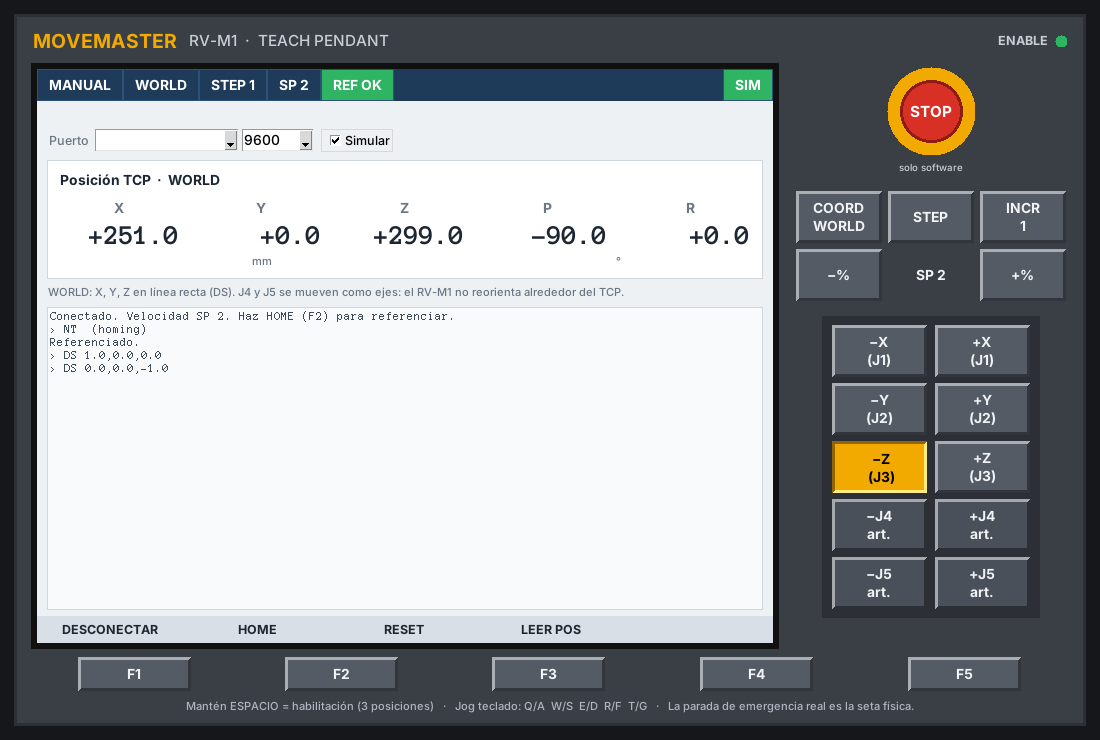
\includegraphics[width=0.8\linewidth]{../docu/pendant.png}
  \caption{Teach pendant de software en modo simulación, tras el homing y con coordenadas WORLD. La barra de estado muestra el modo de operación, el sistema de coordenadas, el incremento de jog, el nivel de velocidad y los estados de referencia y de conexión.}
  \label{fig:pendant}
\end{figure}

En coordenadas articulares (JOINT) cada par de teclas envía un \texttt{DJ} a una articulación; en coordenadas cartesianas (WORLD) los tres primeros pares envían \texttt{DS} según $X$, $Y$ y $Z$, y los dos últimos mueven J4 y J5 como articulaciones, ya que el RV-M1 no reorienta la herramienta alrededor del TCP. El jog puede ser por pasos de 0,1, 1 o 5 unidades (mm o grados) o continuo, con un paso de 2 unidades cada 200~ms mientras se mantiene la tecla y solo si la cola está casi vacía.

Por otro lado, se reproducen por software varias seguridades de los pendants industriales. En primer lugar, la barra espaciadora actúa como dispositivo de validación (\textit{enabling device}): al soltarla se detiene el jog y se vacía la cola. En segundo lugar, el modo WORLD queda bloqueado hasta completar \texttt{NT}, y un error de modo~I devuelve el pendant al estado no referenciado. En tercer lugar, la velocidad se fija en el nivel 2 al conectar y tras una parada, con un aviso a partir del nivel 6. Por último, el botón STOP vacía la cola y bloquea el jog hasta su rearme. Este botón solo deja de enviar comandos, ya que el RV-M1 no puede abortar un movimiento por RS-232C; la parada de emergencia sigue siendo la seta física de la controladora o de la T/B-M1.

Para las pruebas sin robot, el pendant incluye un simulador (MockRVM1) con la misma interfaz que el módulo serie, que reproduce el homing, las lecturas de \texttt{WH} y \texttt{ER} y el error de modo~II de \texttt{DS} sin homing con un modelo cinemático simplificado. Por ello sirve para comprobar la lógica de la interfaz y no los movimientos del brazo. \FALTA{resultado de la prueba del pendant con el robot real conectado al PC.}

\subsection{Placa de interfaz}

El siguiente paso sustituye la conexión directa del PC por una placa de interfaz que actúa como puente RS-232C/MQTT. La placa, un ESP32 o una Raspberry Pi con conversor de niveles RS-232, se conecta a la controladora y a un broker MQTT local. Para ello, traduce los comandos MQTT a comandos del RV-M1, los serializa en una cola, comprueba la controladora con \texttt{ER} y publica el estado y la posición del robot según el protocolo de la \cref{sec:mqtt}. De esta forma, los clientes solo hablan MQTT y el enlace serie queda en un único elemento. \FALTA{modelo de placa, conversor RS-232, broker MQTT y red utilizados.}

\subsection{Gemelo digital}

El gemelo digital es el componente del sistema que sustituye al brazo físico y a su controladora, y se encuentra en desarrollo. Comparte exactamente el contrato MQTT de la placa de interfaz y solo cambia el destino (\texttt{gemelo} en lugar de \texttt{real}), con una instancia por alumno si es necesario. Es decir, reproduce el comportamiento de la controladora visto desde el contrato: homing, jog articular y cartesiano, acuses de recibo, estado y posición. Por tanto, un programa puede probarse sobre el gemelo digital y ejecutarse después sobre el robot físico cambiando solo el destino (\cref{sec:mqtt}). La fidelidad del gemelo digital se medirá frente al robot real. \FALTA{herramienta de implementación, modelo cinemático y detalles de implementación del gemelo digital.}

\section{Protocolo de comunicación MQTT}\label{sec:mqtt}

La comunicación entre el puente RS-232C/MQTT y sus clientes (teach pendant, programas de alumnos, aplicaciones de supervisión y gemelo digital) se define mediante un contrato (versión 0.1, borrador) que fija los topics, el formato de los mensajes y el comportamiento del puente. La regla de diseño es que un cliente solo controla el robot publicando en el topic de comandos; el resto de topics los publica únicamente el puente. Los mensajes son objetos JSON en UTF-8, y \texttt{ts} es una marca de tiempo en milisegundos desde la época Unix.

\subsection{Estructura de topics: robot físico y gemelo digital}

Todos los topics comparten el prefijo \texttt{rvm1/<destino>/<id\_robot>/}, donde \texttt{<destino>} es \texttt{real} para el brazo físico y \texttt{gemelo} para el gemelo digital, y \texttt{<id\_robot>} identifica un robot o una instancia del gemelo digital, por ejemplo por alumno (\texttt{rvm1/gemelo/07/}). La placa de interfaz solo se suscribe a \texttt{rvm1/real/...} y el gemelo digital solo a \texttt{rvm1/gemelo/...}; como los mensajes son idénticos, pasar un programa del gemelo digital al robot físico solo requiere cambiar el destino.

Los cinco topics de cada robot se recogen en la \cref{tab:topics}. Los comandos y los acuses de recibo (\textit{acknowledgements}, ACK) usan QoS~1 para no perder órdenes, y los comandos nunca se retienen, ya que se volverían a ejecutar al reconectar la placa. Por otro lado, el estado, la posición y la conexión sí se retienen, de modo que un cliente que se conecta más tarde recibe los últimos valores. La posición usa QoS~0, ya que se publica periódicamente. Por último, el topic \texttt{online} es la última voluntad (\textit{last will and testament}, LWT) de la placa, así que el broker publica \texttt{"offline"} si la placa se desconecta de forma inesperada.

\begin{table}[t]
  \centering
  \caption{Topics MQTT de un robot, con \texttt{rvm1/real/01/} como prefijo. Los mismos topics existen bajo \texttt{rvm1/gemelo/<id\_robot>/} para el gemelo digital.}
  \label{tab:topics}
  \small
  \begin{tabular}{@{}llccl@{}}
    \toprule
    Topic & Sentido & QoS & Retain & Contenido \\
    \midrule
    \texttt{comandos}         & cliente $\rightarrow$ placa  & 1 & no & Orden a ejecutar \\
    \texttt{comandos/ack}     & placa $\rightarrow$ cliente  & 1 & no & Acuse de cada orden \\
    \texttt{actuadores}       & placa $\rightarrow$ clientes & 1 & sí & Estado actual del robot \\
    \texttt{posicion/mundo}   & placa $\rightarrow$ clientes & 0 & sí & Posición cartesiana del TCP \\
    \texttt{online}           & placa $\rightarrow$ clientes & 1 & sí & \texttt{"online"}/\texttt{"offline"} (LWT) \\
    \bottomrule
  \end{tabular}
\end{table}

\subsection{Comandos y acuses de recibo}

Cada comando contiene un identificador \texttt{id} elegido por el cliente, \texttt{ts}, \texttt{destino}, el nombre \texttt{cmd} y sus argumentos \texttt{args}. El conjunto es deliberadamente reducido y cada comando se corresponde con uno del RV-M1: \texttt{home} se traduce en \texttt{NT}, \texttt{jog\_articular} (articulación 1--5 y grados) en \texttt{DJ}, \texttt{jog\_mundo} (incrementos $dx$, $dy$, $dz$ en milímetros) en \texttt{DS}, \texttt{mover\_pose} ($x$, $y$, $z$, pitch y roll absolutos) en \texttt{MP}, \texttt{velocidad} (nivel 0--9) en \texttt{SP}, \texttt{pinza} en \texttt{GO} o \texttt{GC}, y \texttt{reset} en \texttt{RS}. El comando \texttt{parar} no tiene equivalente en el RV-M1: vacía la cola de la placa, pero no aborta el movimiento en curso.

Cada comando recibe dos ACK en el topic \texttt{comandos/ack}, ambos con el \texttt{id} del comando. El primero se envía al recibirlo, con el estado \texttt{aceptado} si es válido y se ha encolado, o \texttt{rechazado} junto con un campo \texttt{motivo}: destino que no coincide (\texttt{destino}), JSON no válido, comando desconocido o argumento fuera de rango (\texttt{formato}), comando antiguo (\texttt{caducado}), comando cartesiano sin homing (\texttt{no\_referenciado}), robot en error (\texttt{error\_activo}) o sin comunicación con la controladora (\texttt{desconectado}). El segundo ACK se envía al terminar el comando, con el estado \texttt{hecho} si \texttt{ER} devuelve 0 o \texttt{error} si devuelve 1 o 2, e incluye el valor de \texttt{ER}.

El ACK \texttt{hecho} supone que la controladora no responde a \texttt{ER} hasta terminar el movimiento anterior. \VERIFICAR{que la controladora no responde a \texttt{ER} hasta terminar el movimiento anterior; si no se cumple, el ACK \texttt{hecho} debe basarse en otro criterio.} Los rangos de los argumentos también están pendientes de comprobar. \VERIFICAR{rangos válidos de los argumentos de cada comando.}

\subsection{Estado y posición cartesiana del robot}

El topic \texttt{actuadores} describe el estado del robot visto por la placa; se publica en cada cambio y al menos una vez por segundo, y contiene los campos \texttt{conectado} (comunicación RS-232C con la controladora), \texttt{referenciado} (homing completado sin error desde el último arranque o error de modo~I), \texttt{error} (último valor de \texttt{ER}), \texttt{velocidad} (último \texttt{SP} enviado), \texttt{pinza} (última orden de la pinza, o desconocida), \texttt{ocupado} (hay un comando enviado al robot sin terminar) y \texttt{cola} (comandos pendientes en la placa). Como la controladora no informa del estado de cada motor (corriente, temperatura o ángulo), el topic describe el robot en su conjunto y no cada actuador.

El topic \texttt{posicion/mundo} contiene la posición cartesiana del TCP leída con \texttt{WH}: $x$, $y$ y $z$ en milímetros y pitch y roll en grados. Se publica tras cada movimiento y cada 500~ms en reposo, e incluye el campo \texttt{valida}, falso mientras el robot no está referenciado, ya que sin homing la posición no es fiable. \FALTA{frecuencia de publicación real alcanzada y latencias medidas (de los experimentos).}

\subsection{Mecanismos de seguridad}

El protocolo añade varias comprobaciones antes de que un comando llegue a la controladora. En primer lugar, el campo \texttt{destino} debe coincidir con el del receptor, una segunda comprobación tras el topic para no mover por error el brazo físico con un programa del gemelo digital. En segundo lugar, un comando con más de 500~ms de antigüedad se rechaza como \texttt{caducado}, de modo que un jog retrasado por la red no mueve el robot tarde. Para ello, los relojes de clientes y placa deben estar sincronizados. \FALTA{mecanismo de sincronización de relojes entre clientes y placa (p.~ej., NTP).} En tercer lugar, \texttt{jog\_mundo} y \texttt{mover\_pose} se rechazan mientras el robot no está referenciado, como en el modo WORLD del teach pendant, y cualquier movimiento se rechaza con el robot en error hasta recibir un \texttt{reset}. Por último, la pérdida de comunicación con la controladora se indica con \texttt{conectado} y el motivo \texttt{desconectado}, y la de la propia placa con la LWT de \texttt{online}.

Al igual que en el teach pendant, estos mecanismos solo controlan qué comandos se envían. Por tanto, como \texttt{parar} no detiene un movimiento iniciado, la parada de emergencia física de la controladora o de la T/B-M1 sigue siendo el único medio para detener el brazo de forma inmediata.

\section{Experimentos y resultados}\label{sec:experiments}
\subsection{Montaje experimental}
\FALTA{Montaje, red, versiones de código y contrato.}
\subsection{Resultados}
\FALTA{Solo con datos de analisis/ tras ejecutar los experimentos con el robot real.}
\subsection{Discusión}
\FALTA{Limitaciones y aplicabilidad a otros equipos con puerto serie.}

\section{Conclusiones}\label{sec:conclusions}
\FALTA{Escribir tras los resultados (incluye trabajo futuro).}

\section*{Disponibilidad de código y datos}
El código fuente, el contrato MQTT, los protocolos experimentales y los datos en bruto están disponibles en \url{https://github.com/AlvarLegaz/modernizacion-robot-rv-m1} \FALTA{DOI de Zenodo de la versión usada}.

\section*{Uso de herramientas de inteligencia artificial}
\FALTA{Declaración según la política de la revista: herramientas usadas (asistente de IA para búsqueda bibliográfica, borradores y código), y que el autor revisó y asume la responsabilidad de todo el contenido.}

\section*{Financiación}
Este trabajo no ha recibido financiación externa.

\section*{Conflicto de intereses}
El autor declara que no existe conflicto de intereses.


\bibliographystyle{plainnat}
\bibliography{../referencias/refs}

\end{document}
